% Generated file: held-out test MAPE (pure TikZ)
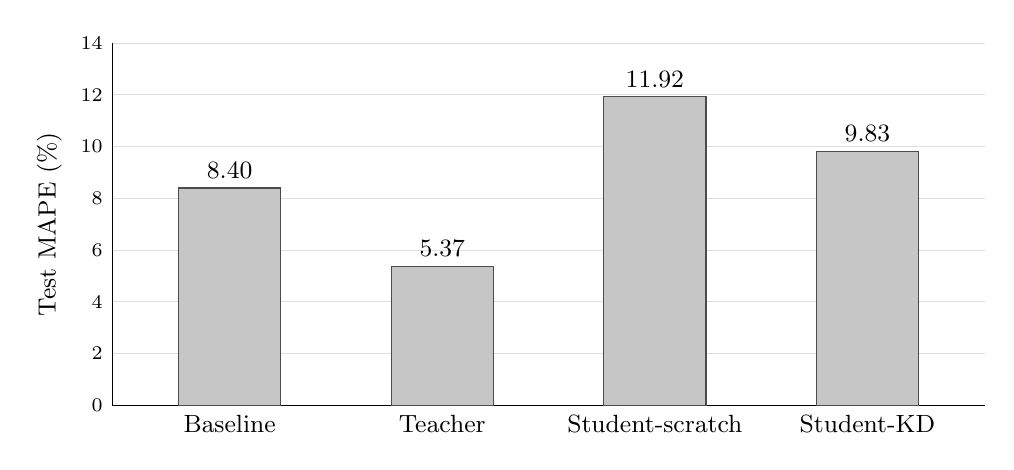
\begin{tikzpicture}[font=\small]
\draw[gray!25] (0,0.000) -- (11.080,0.000);
\node[left,font=\scriptsize] at (0,0.000) {0};
\draw[gray!25] (0,0.657) -- (11.080,0.657);
\node[left,font=\scriptsize] at (0,0.657) {2};
\draw[gray!25] (0,1.314) -- (11.080,1.314);
\node[left,font=\scriptsize] at (0,1.314) {4};
\draw[gray!25] (0,1.971) -- (11.080,1.971);
\node[left,font=\scriptsize] at (0,1.971) {6};
\draw[gray!25] (0,2.629) -- (11.080,2.629);
\node[left,font=\scriptsize] at (0,2.629) {8};
\draw[gray!25] (0,3.286) -- (11.080,3.286);
\node[left,font=\scriptsize] at (0,3.286) {10};
\draw[gray!25] (0,3.943) -- (11.080,3.943);
\node[left,font=\scriptsize] at (0,3.943) {12};
\draw[gray!25] (0,4.600) -- (11.080,4.600);
\node[left,font=\scriptsize] at (0,4.600) {14};
\draw (0,0) -- (11.080,0); \draw (0,0) -- (0,4.600);
\fill[gray!45, draw=black!70] (0.840,0) rectangle (2.140,2.760);
\node[above,font=\small] at (1.490,2.760) {8.40};
\node[below,font=\small] at (1.490,0) {Baseline};
\fill[gray!45, draw=black!70] (3.540,0) rectangle (4.840,1.766);
\node[above,font=\small] at (4.190,1.766) {5.37};
\node[below,font=\small] at (4.190,0) {Teacher};
\fill[gray!45, draw=black!70] (6.240,0) rectangle (7.540,3.918);
\node[above,font=\small] at (6.890,3.918) {11.92};
\node[below,font=\small] at (6.890,0) {Student-scratch};
\fill[gray!45, draw=black!70] (8.940,0) rectangle (10.240,3.229);
\node[above,font=\small] at (9.590,3.229) {9.83};
\node[below,font=\small] at (9.590,0) {Student-KD};
\node[rotate=90] at (-0.8,2.300) {Test MAPE (\%)};
\end{tikzpicture}
